Die Serverzuständigkeiten lassen sich in folgende Aspekte zusammenfassen:
\begin{itemize}
\item Empfangen und Beantworten der Clientanfragen
\item Routing der Anfragen zu den entsprechenden Abhandlungsroutinen
\item Überprüfen der Identität des Clients
\item Kommunikation zur Datenbank für die persistente Speicherung der Zustände der Nutzer und ihrer Präferenzen, Swipes und Matches.
\item Matching-Algorithmus
\end{itemize} 

In den folgenden Unterkapitel ....

\subsubsection{Webserver}
\paragraph{Bereitstellung des Webservers}
Zunächst wird das Node.js-Installationspaket aus der offiziellen Seite der Hersteller heruntergeladen und ausgeführt. Hierbei werden sowohl die Laufzeitumgebung für Node.JS, als auch der npm package manager installiert [Siehe nächste Abbildung]. 
Der Paket-Manager npm (ehemals Node Package Manager) dient der Verwaltung der Node.js-Module. 
Zusätzlich wird bei der Installation ausgewählt, dass Node.js sowie npm und dessen Module zu den Umgebungsvariablen hinzugefügt werden. Dabei werden Variablen unter ihrem Applikationsnamen gespeichert und ihre entsprechende Datei-Pfade hinterlegt.
Über den Zugriff auf diese Umgebungsvariable ist ein schneller Zugriff über ein Terminal beziehungsweise einer anderen Applikation gewährleistet.


\begin{figure}[h]
\centering
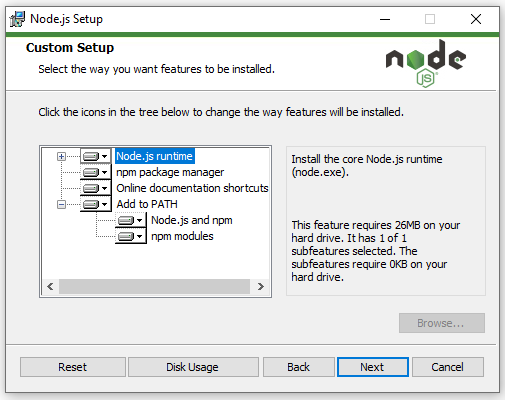
\includegraphics[width=10cm]{images/nodejs_install.png}
\caption{Node.JS Installation}
\end{figure}

Nach der Installation von Node.js kann das Projekt mithilfe des Befehls „npm init“ im Terminal initializiert werden. 
Hier werden nacheinander Input für relevante Projektaspekte wie dem Projektnamen, der Initialversion, der Startprogrammdatei oder dem GIT-Repository abgefragt.  
Im Anschluss wird im aktuellen Verzeichnis eine Datei „package.json“ erstellt,  bei der es sich um eine Manifest-Datei im JSON- Format handelt, die unter anderem die benötigten Pakete sowie dessen Version, als auch projektspezifische Meta-Informationen wie den Projektnamen, der Projektversion, der Projektbeschreibung und dem Author enthält.
\newline
Im Anschluss an die Initialisierung werden die benötigten Pakete installiert. Dafür wird der Befehl „npm install“ in Kombination mit dem angeforderten Modul genutzt. 
Nach der ersten Installation eines Moduls wird im Hauptverzeichnis des Projekts automatisch ein Ordner „node\_modules“ erzeugt. Dieser enthält die Quelldaten der Node.js-Module. 
\newline
Da die Funktionalität, die nodemon bietet, nur in der Entwicklung benötigt wird, wird in der Datei „package.json“ ein Entwicklungsskript „devStart“ definiert. 
Skripte erlauben das automatische Starten von anderen Applikationen. Über „npm run“ in Kombination mit dem auszuführenden Skript wird die Hauptapplikation über die Datei, die im package.json unter „main“ hinterlegt ist, zusammen mit den Applikationen, die im package.json unter dem entsprechenden Skript aufgezählt sind, gestartet.
\newline
Als Applikationsstartpunkt wird die Datei „server.js“ erzeugt und im package.json unter main hinterlegt. 

\begin{lstlisting}[caption=Datei package.json, label=lst:packagejson]
 {
  "name": "StreamSwipeServer",
  "version": "1.0.0",
  "description": "Our Backend-Server for the StreamSwipe Mobile Application",
  "main": "server.js",
  "scripts": {
    "start": "",
    "devStart": "nodemon"
  },
  "author": "Robin Meckler, Vincent Schreck, Leon Gieringer",
  "license": "-",
  "dependencies": {
    "express": "^4.17.1",
    "firebase-admin": "^9.5.0",
    "mongoose": "^5.11.17",
    "node-cron": "^2.0.3",
    "dotenv": "^8.2.0"
  },
  "devDependencies":{
    "nodemon": "^2.0.7"
  }
}
\end{lstlisting}

\paragraph{Sichere Kommunikation}

Das http-Modul ermöglicht eine Kommunikation über das http-Protokoll. 
\begin{lstlisting}[caption=Einfache Verbindung, label=lst:nodejs_easyconnection]
 {
 	const app = express();
	app.use(express.json()); 
 	var httpServer = http.createServer(app);
 	httpServer.listen(process.env.HTTP_PORT, () => 
 	console.log("HTTP-Server started on " + process.env.HTTP_PORT));
}
\end{lstlisting}

Dabei werden jedoch die Daten unverschlüsselt versendet. Um ausreichend Datenschutz zu gewährleisten, wird stattdessen das https-modul genutzt. []%[https://nodejs.org/api/https.html]
\newline
Benötigt für einen HTTPS-Server werden ein Sicherheitszertifikat und ein privater Schlüssel, die zunächst mithilfe des Tools OpenSSL erzeugt werden.  
Dabei ist zu beachten, dass während der Entwicklungsphase das Zertifikat nicht von einer zuständigen Zertfikatsstelle signiert wird und somit von anderen Gegenstellen nicht akzeptiert wird. => TODO Frondendkommunikation, Ausblick
\newline
In der Anwendung wird zunächst ein Objekt "httpsOptions" erzeugt, dass unter dem Attribut "cert" das generierte Sicherheitszertifikat und unter dem Attribut "key" den privaten Schlüssel enthält. Anschließend wird über die Funktion "createServer" des https-Objekts der https-Server gestartet, woraufhin ein Objekt vom Typ https.Server zurückgegeben wird. []
 %[https://nodejs.org/api/https.html#https_class_https_server] 
Diesem Serverobjekt wird über seine Methode "listen" aufgefordet, auf eingehende Nachrichten in dem als Parameter übergebenem Port einzugehen.

\begin{lstlisting}[caption=Gesicherte Verbindung, label=lst:nodejs_safeconnection]
 {
 	...
	const https = require("https");
	const httpsOptions = {
	  cert: fs.readFileSync('sslcert/server.crt', 'utf8'),
	  key: fs.readFileSync('sslcert/server.key', 'utf8')
	}
	var httpsServer = https.createServer(httpsOptions, app);
	httpsServer.listen(process.env.HTTPS_PORT, () => {console.log("HTTPS - 	Server started on " + process.env.HTTPS_PORT)});
}
\end{lstlisting}

\subsubsection{Datenbank}
\paragraph{Bereitstellung der Datenbank}
=> MongoDB 
=> WiredTiger Engine, Replica Sets

\paragraph{Datenbankverbindung}
Wie bereits erwähnt, wird das Modul „mongoose“ für die Verbindung mit der MongoDB-Datenbank verwendet. 
Da der Quellcode in anderen Dateien hinterlegt ist, muss für den Zugriff auf dessen Funktionalitäten das entsprechende Modul zunächst inkludiert werden. Dazu wird die require-Methode aufgerufen, die ein Objekt zurückgibt, dass die aus dem Modul exportierten Methoden enthält und im Folgenden als Variabel mit dem Namen „mongoose“ gespeichert wird. 
\newline
Über die connect-Methode des zurückgelieferten Objekts wird nun bei Parameterübergabe der URL der Datenbank versucht, eine Verbindung aufzubauen.  
Dabei wird unter der Objekt-Membervariabel  „connection“ ein Objekt vom Typ „Connection“ hinterlegt, über das bei erfolgreicher Verbindung mit der Datenbank kommuniziert werden kann und das nachfolgend unter der Variabel „database“ abgespeichert ist. 

\begin{lstlisting}[caption=Verbindung zur MongoDB-Datenbank, label=lst:mongodbconnection]
 {
 	const mongoose = require('mongoose');
	let database = null;

	async function startDatabase() {
	await mongoose.connect(process.env.DATABASE_URL, 
	{useNewUrlParser: true,
	useUnifiedTopology: true}); 
  	database = mongoose.connection;
  	database.on('error',(error) => console.log(error));
  	database.on('open',(error) => console.log('Connected to DB'))
	}

	async function getDatabase() {
 	 	if (!mongoose.connection) await startDatabase();
  		return database;
	}

	module.exports = {
  		getDatabase,
  		startDatabase,
	}
}
\end{lstlisting}

\paragraph{Datenbankmodelle und Schemata}

Ein Model in Mongoose ist ein aus einer Schemadefinition erstellter Konstruktor, aus denen Objekte instanziiert werden können. Diese Instanzen stehen in direkter Verbindung zu den jeweiligen Collections der verbundenen Datenbank und enthalten Methoden für die persistente Speicherung, Bearbeitung oder Löschung.
\newline
Folgender Code zeigt den Aufbau des Schemas für die Swipe-Collection. 

\begin{lstlisting}[caption=Swipe Schema und Model, label=lst:modelswipe]
	const mongoose = require('mongoose')

	const swipeSchema = new mongoose.Schema({
    uid: {
        type: String,
        required: true
    },
    swipes :
     [{ movieid: { type: String },
        swipeaction: {type: Number}}]
	})

	module.exports = mongoose.model('Swipe',swipeSchema)
\end{lstlisting}

Die einzelnen Schemata wurden nach dem im Konzept beschriebenen Aufbau der Datensätze[TODO] in separaten Dateien unter dem Verzeichnis '/database/models' erstellt. Jede Datei exportiert dabei das aus dem zugehörigen Schema erzeugten Model.

\paragraph{Datenbankzugriff}
